% Incluye el preambulo.
\IfFileExists{preamble.fmt}{}{\documentclass
[
  12pt,
  letterpaper,
  openany,
  oneside,
  draft
]{book}

\ExplSyntaxOn
\makeatletter

\RequirePackage { geometry }
\RequirePackage { setspace }
\RequirePackage [ spanish ] { babel }
\RequirePackage [ tracking=smallcaps, babel=true, disable=ifdraft ] { microtype }
\RequirePackage { enumitem }
\RequirePackage { csquotes }
\RequirePackage { biblatex }
\RequirePackage { xcolor }
\RequirePackage { graphicx }
\RequirePackage { mathtools, amsthm }
\RequirePackage { dirtytalk }
\RequirePackage { epigraph }
\RequirePackage { hyperref }
\RequirePackage [ spanish ] { cleveref }
\RequirePackage { lineno }

% Cref
\crefname{section}{\S}{\S}

% Set page margins
\geometry
    {
        includehead,
        paper = letterpaper,
        left = 3cm,
        right = 2cm,
        bottom = 2cm,
        top = 2cm,
        marginparsep = 10pt,
        marginparwidth = 2cm,
    }

% Set fonts
\usepackage[T1]{fontenc}
\usepackage{mlmodern}
\usepackage[cal=boondoxo, calscaled=1.05, frak=euler]{mathalfa}
% Patch bold font
\renewcommand{\bfdefault}{b}
\DeclareRobustCommand\bfseries
        {\not@math@alphabet\bfseries\mathbf
         \fontfamily{lmr}\fontseries\bfdefault\selectfont}
\newcommand{\titlefont}{\bfseries\selectfont}

% Set basic spacing
\setlength { \parindent } { 8.46pt }
\setlength { \parskip } { 6pt }
\onehalfspacing

% Headers and footer
\pagestyle{headings}
\gdef\@oddhead{\hfil\thepage}

% Bibliography
\addbibresource{references.bib}

% Hyperref
\hypersetup
    {
        colorlinks = true,
        allcolors = black,
    }

% Theorems
\newtheoremstyle{teo}% hnamei
    {.5\baselineskip}% hSpace abovei
    {.5\baselineskip}% hSpace belowi
    {}% hBody fonti
    {}% hIndent amounti
    {\scshape}% hTheorem head fonti
    {.}% hPunctuation after theorem headi
    {.5em}% hSpace after theorem headi
    {}% hTheorem head spec (can be left empty, meaning ‘normal’)i
\theoremstyle{teo}
\newtheorem{defi}{Definición}[chapter]
\newtheorem{lem}{Lema}[chapter]
\newtheorem{teo}{Teorema}[chapter]
\newtheorem{cor}{Corolario}[chapter]

% QED symbol
\renewcommand\qedsymbol{\rule{.30em}{1.9ex}}

% Sectioning commands
\usepackage[explicit]{titlesec}
\titleformat
    {\chapter}
    [display]
    {\titlefont}
    {
        \centering
        \fontsize{14}{14}\selectfont
        \UpperCase{Capítulo}~\thechapter\\[10pt]
        \fontsize{12}{12}\selectfont
        \UpperCase{#1}
    }
    {0ex}
    {\centering}
\titleformat{name=\chapter, numberless}
    [block]
    {\titlefont}
    {\fontsize{14}{14}\selectfont\UpperCase{#1}}
    {0ex}
    {\centering}
\titleformat
    {\section}
    {\titlefont}
    {\thesection\fontsize{12}{12}\selectfont\ #1}
    {0ex}
    {}
\titleformat{name=\section, numberless}
    [block]
    {\titlefont}
    {\fontsize{12}{12}\selectfont #1}
    {0ex}
    {}

% USB logo
\cs_set_eq:NN \latex_centering:D \centering

\cs_new:Npn \th_print_logo_head:n #1
    {
        \group_begin:
            \latex_centering:D
            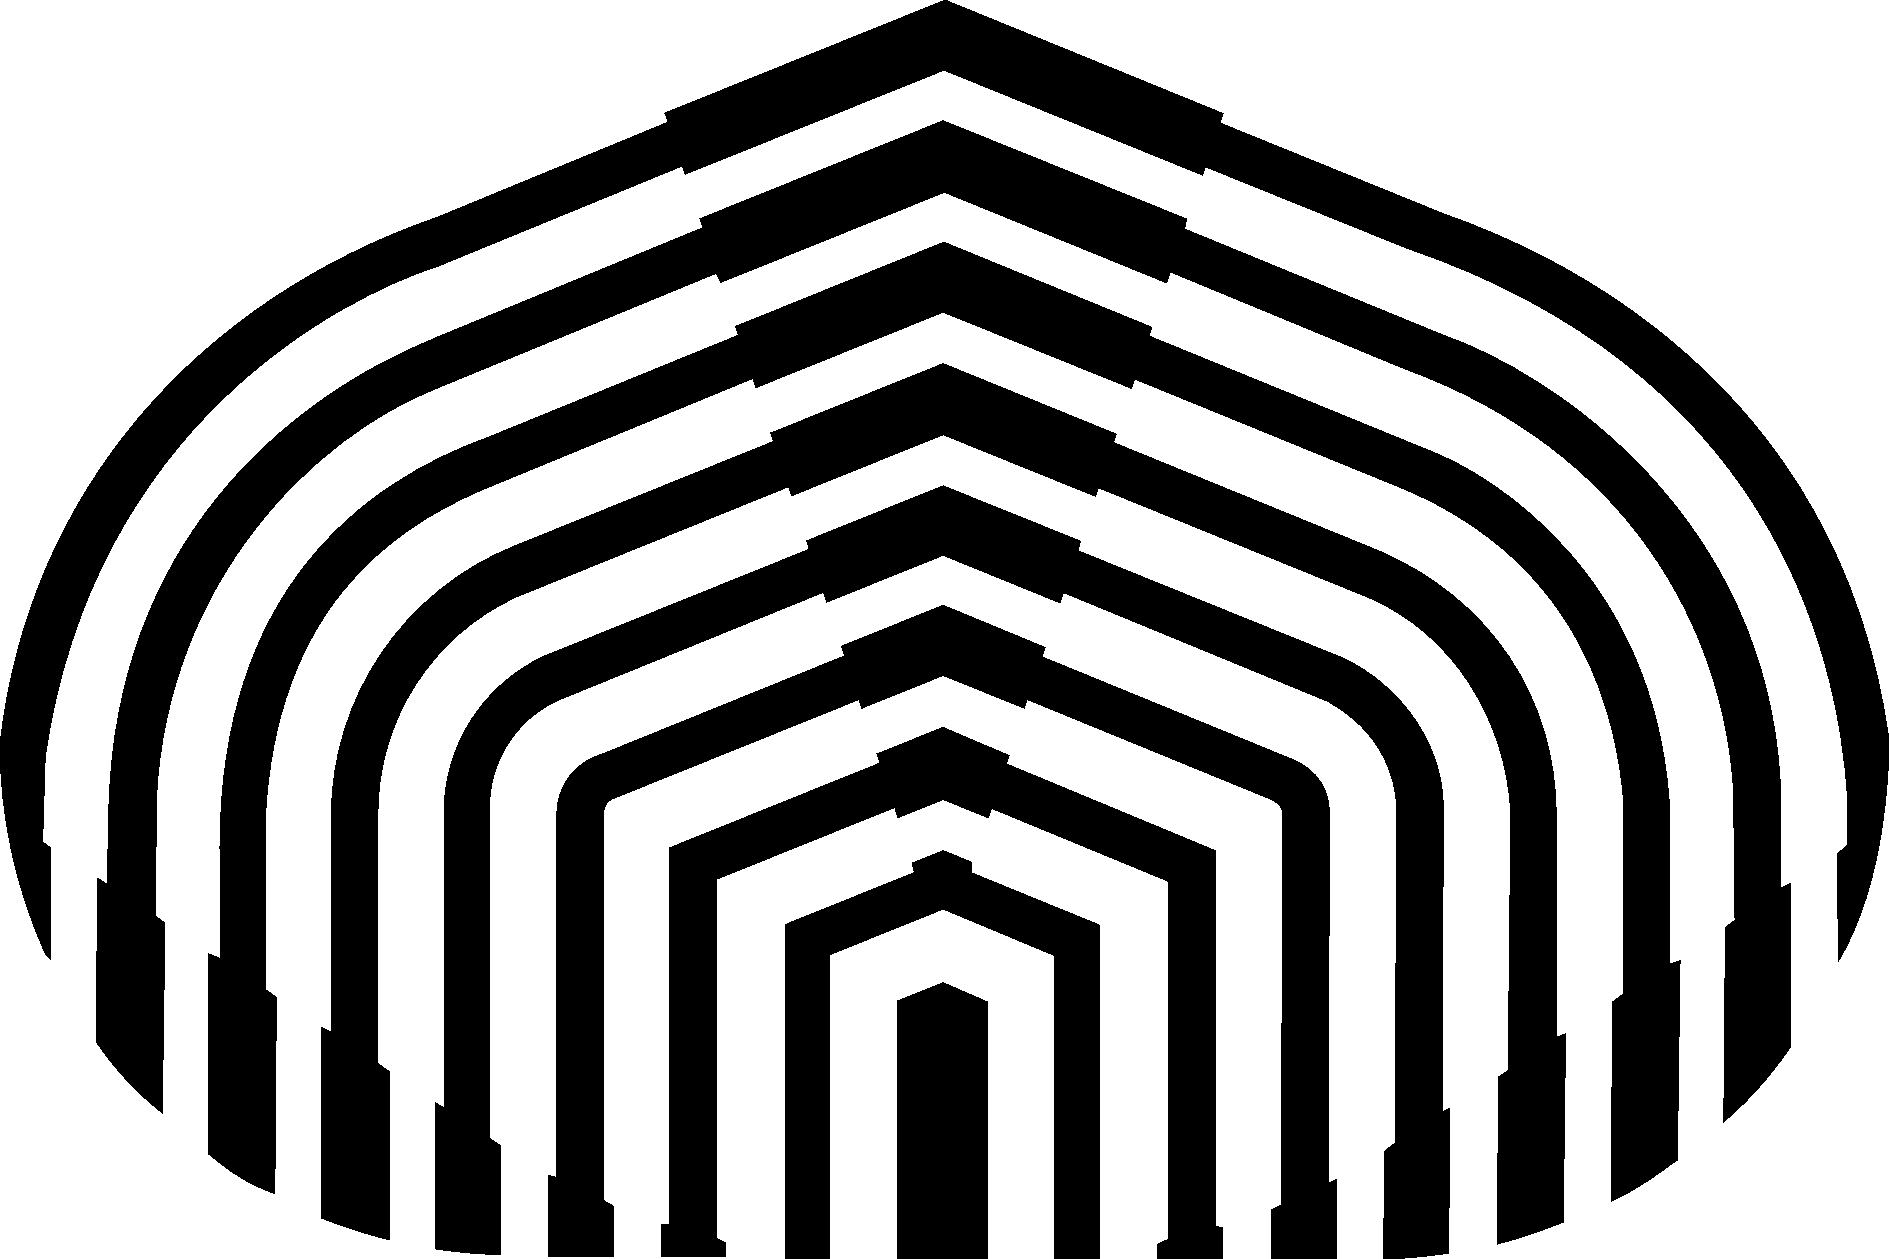
\includegraphics[scale=.3]{resources/usblogo} \\
            { \titlefont \UpperCase{#1} }
            \tex_par:D
        \group_end:
    }

\NewDocumentCommand{ \UpperCase }{ m }
    {
        \group_begin:
        \lsstyle
        \text_uppercase:n { #1 }
        \group_end:
    }

\NewDocumentCommand{ \UppercaseBold }{ m }
    {
        { \titlefont\UpperCase{#1} }
    }

\NewDocumentCommand{ \PrintUsbLogo }{ m }
    {
        \th_print_logo_head:n { #1 }
    }

\NewDocumentCommand{ \ToC }{}
    {
        \chapter*{Índice~General}
        \@starttoc{toc}
    }

% Notes
\reversemarginpar
\NewDocumentCommand{ \note }{ m }
{
    \@ifclasswith{ book } { draft }
    {
        \begingroup
            \color{blue}
            \sffamily
            \small
            \textlangle #1 \textrangle
        \endgroup
    } {}
    \PackageWarning{Notes}{Revisar~nota}
}

% Wrapping
\newlength{\wrapwd}
\NewDocumentCommand { \wrapto } { o o m }
{
    \IfNoValueTF { #1 }
        { \setlength{\wrapwd}{.6\linewidth} }
        { \setlength{\wrapwd}{#1} }
    \IfNoValueTF { #2 }
        { \let\wrapal\raggedright }
        { \let\wrapal#2 }
    \begin{minipage}{\wrapwd}
        \wrapal
        #3
    \end{minipage}
}

% Conditionals
\newif { \ifcaratula }
\newif { \ifpaginatitulo }
\newif { \ifresumen }
\newif { \ifdedicatoria }
\newif { \ifagradecimientos }
\newif { \iftoc }
\newif { \ifsimbolos }
\newif { \ifabreviaturas }
\newif { \ifintro }
\newif { \ifbasicos }
\newif { \ifreferencias }

\@ifclasswith{ book } { draft }
{
  \AddToHook{begindocument}
  {
    \newbox{\watermark}
    \savebox{\watermark}
    {
      \rotatebox{45}
      {
        \scalebox{7}
        {
          \textcolor{red!5}{BORRADOR}
        }
      }
    }
    \AddToHook{ shipout/background }
    {
      \put (\paperwidth/2 - \wd\watermark/2,-\paperheight/2 - \ht\watermark/2)
      {
        \usebox{\watermark}
      }
    }
  }
}{}

% macros
\newcommand { \MainTitle }
    {
        Estudio~comparativo~de~tres~demostraciones~
        del~teorema~de~inconsistencia~de~Kunen.
    }

\newcommand { \autor }
    {
        Jhonny~Lanzuisi~Berrizbeitia
    }

\newcommand { \tutor }
    {
        Jesús~Nieto~Martínez
    }

\newcommand { \coord }
    {
        Matemáticas
    }

\DeclareMathOperator{\Con}{Con}
\DeclareMathOperator{\Crit}{crit}

\NewDocumentCommand { \model } { m }
{
    \mathfrak { #1 }
}
\NewDocumentCommand { \set } { m }
{
    \left\{ #1 \right\}
}
\NewDocumentCommand { \lex } { m }
{
    \mathcal { #1 }
}
\NewDocumentCommand { \crit } { m }
{
    \Crit (\, #1\, )
}

\NewDocumentCommand { \pwset } { m }
{
    \mathcal{P}(#1)
}

\NewDocumentCommand{ \concept } { m }
{
    \emph{#1}
}

\NewDocumentCommand{ \op } { m }
{
     \langle #1 \rangle
}

\NewDocumentCommand{ \seq } { m }
{
     \langle #1 \rangle
}

\NewDocumentCommand{ \con } { m }
{
    \Con ( #1 )
}

\NewDocumentCommand { \cna } { m }
{
    \str_if_eq:nnTF { #1 } { . } { c.\,n.\,a. } { c.\,n.\,a.#1 }
}

\DeclareMathOperator*{ \dint } { \bigtriangleup }
\DeclareMathOperator*{ \cf } { cf }

\@ifclasswith{ book } { draft } { \linenumbers } {}
\makeatother
\ExplSyntaxOff
\dump
}

% Secciones a incluir.
\caratulafalse
\paginatitulotrue
\resumenfalse
\dedicatoriafalse
\agradecimientosfalse
\listastrue
\toctrue
\introfalse
\referenciastrue
\basicostrue

\begin{document}
% ------------------------------------------------------------------------------
%                                 FRONTMATTER.
% ------------------------------------------------------------------------------
\frontmatter
% ------------------------------------------------------------------------------
% Caratula.
% ------------------------------------------------------------------------------
\ifcaratula\newpage
WIP: CARATULA.
\fi
% ------------------------------------------------------------------------------
% Página de Título.
% ------------------------------------------------------------------------------
\ifpaginatitulo\newpage
\bgroup
    \centering
    \thispagestyle{empty}

    \PrintUsbLogo
    {
        Universidad Simón Bolívar\\
        Decanato de estudios profesionales\\
        Coordinación de \coord
    }

    \vspace{1.5cm}

    \UppercaseBold{
        \wrapto[14cm][\centering]
        {\MainTitle}
    }

    \vspace{1.5cm}

    Por:
    \\
    \autor

    \vspace{1.5cm}

    Realizado con la asesoría de:
    \\
    \tutor

    \vspace{3cm}

    \MakeUppercase{Proyecto de Grado}\\
    Presentado ante la Ilustre Universidad Simón Bolívar\\
    como requisito parcial para optar al título de\\
    Licenciatura en Matemáticas Puras

    \vspace{\fill}

    \textbf{Sartenejas, \today}\par
\egroup
\fi
% ------------------------------------------------------------------------------
% Resumen.
% ------------------------------------------------------------------------------
% TODO: reescribir mencionando las 3 demostraciones
\ifresumen\newpage
\PrintUsbLogo
    {
        Universidad Simón Bolívar\\
        Decanato de estudios profesionales\\
        Coordinación de \coord
    }

\begin{center}
    \begin{minipage}{14cm}
        \centering
        \UppercaseBold
            {
                \MainTitle
            }
    \end{minipage}

    \vspace{.5cm}

    \UpperCase
        {
            Proyecto de grado
        } \\
    Realizado por: \autor \\
    Con la asesoría de: \tutor \\[.5cm]
    \UppercaseBold{Resúmen}

\end{center}

\note{El titulo menciona 3 demostraciones pero el resumen no dice cuales son.}
El teorema de inconsistencia de Kunen, que establece la inexistencia en
ZFC (teoría de conjuntos Zermelo-Fraenkel con el axioma de elección)
de cualquier inmersión elemental $j\colon V\prec V$ y, por lo tanto, de los cardinales
de Reinhardt, es un resultado central de la teoría de cardinales grandes.
El teorema de Kunen da una cota superior para la jerarquía de los cardinales grandes.

Se tratará el teorema mencionado a través de tres demostraciones, cada una de naturaleza
distinta. El libro de Kanamori \autocite{cohen_independence_1964} es la referencia estándar
en el estudio de los cardinales grandes y la fuente
de dichas demostraciones.

Para poder estudiar el resultado de Kunen en profundidad,
se divide el presente escrito en 3 capítulos más la introducción.
En la introducción se discuten los antecedentes históricos y la importancia
de este teorema.
El primer capítulo consta de nociones básicas necesarias para su enunciación y demostración.
El segundo capítulo introduce nociones también necesarias, pero ya no básicas, como los cardinales
supercompáctos o extendibles.
Para el tercer capítulo, se entra de lleno en el resultado de Kunen y sus demostraciones.

Las conclusiones discuten las posibles vías de investigación y desarrollo en esta área,
haciendo énfasis en un problema abierto asociado al teorema:
¿Seguirá siendo cierto el resultado de Kunen si se prescinde del axioma de elección?

\vspace{\fill}

\textbf{Palabras Clave:}
\fi
% ------------------------------------------------------------------------------
% Dedicatoria.
% ------------------------------------------------------------------------------
\ifdedicatoria\newpage
WIP: DEDICATORIA.
\fi
% ------------------------------------------------------------------------------
% Agradecimientos.
% ------------------------------------------------------------------------------
\ifagradecimientos\newpage
WIP: AGRADECIMIENTOS.
\fi
% ------------------------------------------------------------------------------
% Listas de simbolos y abreviaturas.
% ------------------------------------------------------------------------------
\iflistas
\chapter*{Lista de Símbolos}

En la lista siguiente, $C$ es un conjunto.

\begin{center}
    \begin{tabular}{cl}
        Símbolo & Significado \\
        \hline\noalign{\smallskip}
        $\pwset{C}$ & Conjunto de partes.\\
        $\sup(C)$ & Supremo, es decir, $\bigcup C$.\\
        $\cf C$ & Cofinalidad
    \end{tabular}
\end{center}

\newpage
\chapter*{Lista de Abreviaturas}

\begin{center}
    \begin{tabular}{cl}
        Abreviatura & Significado \\
        \hline\noalign{\smallskip}
        ZF & Teoría de conjuntos de Zermelo-Fraenkel.\\
        AC & Axioma de elección.\\
        ZFC & ZF al añadir AC.\\
        NBG & Teoría de conjuntos de Von Neumann, Bernays y Gödel.\\
        CH & Hipótesis del continuo: $2^{\aleph_0} = \aleph_1$. \\
        \cna{} & Cerrado no acotado. \\
    \end{tabular}
\end{center}
\fi
% ------------------------------------------------------------------------------
% Tabla de contenidos.
% ------------------------------------------------------------------------------
\iftoc \ToC \fi
% ------------------------------------------------------------------------------
% Introducción.
% ------------------------------------------------------------------------------
%     - Conceptos básicos de teoría de conjuntos. Establecer la teoría de conjuntos en la que se va a trabajar y establecer notación.
% Citar CG de ivorra en el parrafo sobre la importancia.
% Mencionar la jerarquía de los CG, y explicar que se tratará una parte superior
% de la jerarquía: de los cardinales medibles para arriba. Quizás dar un breve resúmen
% de como es la jerarquía por debajo. (Los grafos que tiene Ivorra en CG podrían usarse)
\ifintro
\chapter*{Introducción}

\epigraph
{
Del paraíso que Cantor ha creado para nosotros, nadie ha de expulsarnos.
}
{David Hilbert. \autocite[pág 170]{hilbert_uber_1926}}

Las hipótesis de cardinales grandes son los axiomas matemáticos
más fuertes jamás postulados: estipulan la existencia de conjuntos
infinitos de tal tamaño, que no son decidibles en el marco de la teoría de conjuntos.
Los más pequeños entre ellos, siendo enormes, nunca son suficientemente
fuertes para demostrar la existencia de cardinales mayores.
El teorema de inconsistencia de Kunen es
una cota superior que impone el axioma de elección a las
hipótesis de cardinales grandes.
Pero, ¿qué utilidad pueden tener los cardinales grandes?
¿por qué interesa el resultado de Kunen?

La principal razón por la que el estudio de estos conjuntos infinitos
es relevante proviene del siguiente hecho:
es con ellos que cualquier aserción sobre consistencia relativa
puede medirse.
Sabemos gracias a Gödel que si en una teoría se puede desarrollar la aritmética
elemental, esta no puede demostrar su propia consistencia.
Si $T$ es una teoría de esta forma, lo que sí se puede es construir la teoría
$T'=T+\con{T},$
donde añadimos como nuevo axioma la consistencia
de $T$,
que evidentemente demuestra que $T$ es consistente; todo esto sin contradecir
el resultado de Gödel. Pero tenemos ahora un nuevo problema: la consistencia
de $T'$.
Consideremos entonces otra teoría,
\[T'' = T + \con{T} + \con{T + \con{T}},\]
que demuestra la consistencia de $T'$.
Podemos continuar de esta manera, definiendo $T''', T'''',\text{etc}$.
De esta manera se construye una jerarquía análoga a la de los ordinales,
en una torre ascendente infinita de consistencia relativa
\autocite[\S 7.7]{hamkins_lectures_2020}.

La conexión importante es la siguiente:
los cardinales grandes representan una instanciación de esta jerarquía.
Podemos entonces, a través de ellos, estudiar este universo infinito de
consistencia al que Gödel nos abrió las puertas.
Convendría hablar un poco más en detalle sobre los cardinales grandes
y su lugar en la tradición, empezada por Cantor, de la teoría de conjuntos.

\section*{Cardinales Grandes. Extensión hasta la Inconsistencia.}

Los cardinales grandes tienen sus orígenes en las investigaciones cantorianas
sobre conjuntos definibles de números reales y los números transfinitos.
Fue Felix Hausdorff \autocite{hausdorff_grundzuge_nodate}
el primero en considerar un cardinal grande,
los débilmente inaccesibles.
Paul Mahlo \autocite{mahlo_uber_1911,mahlo_zur_1912,mahlo_zur_1913}
postulará después los cardinales que llevan su nombre.
Al considerar la clausura sobre la formación del conjunto de partes,
Sierpiński-Tarski \autocite{sierpinski_sur_1930} y  Zermelo \autocite{zermelo_uber_1930}
llegan a la noción de cardinal (fuertemente) inaccesible.

Stanisław Ulam \autocite{ulam_zur_1930}, al estudiar la medida de Lebesgue,
introduce los cardinales medibles y con ellos la primera
pregunta sobre la jerarquía de los cardinales grandes:
¿Es el primer cardinal inaccesible también medible?
El desarrollo de los cardinales grandes dependerá a partir de este
momento de la incorporación de la teoría de modelos (\cref{sec:models}) en las matemáticas.

La generalización de la lógica de primer orden, obtenida al
permitir una cantidad infinita de operaciones lógicas,
permitió a Tarski \autocite{tarski_problems_1966} definir los cardinales (débil y fuerte)
compactos como una generalización del teorema de compacidad
para estas lógicas. Los cardinales compactos dieron solución
a la pregunta propuesta unos párrafos más arriba:
el primer cardinal inaccesible no es medible.

El siguiente gran salto adelante vendría de la mano de
Paul Cohen \autocite{cohen_independence_1963,cohen_independence_1964}
y la invención del forcing como técnica
para establecer resultados de consistencia relativa.
Cohen usaría su nueva técnica para construir un modelo de la
teoría de conjuntos donde falla la hipótesis del continuo
y junto con un resultado anterior de Gödel---a saber, que
en el universo de los constructibles se verifica CH---%
logra resolver finalmente la gran pregunta de Cantor sobre cardinalidades
intermedias entre los naturales y el continuo.

Finalmente, en la década de 1970,
Solovay y Reinhardt comienzan a postular
hipótesis de cardinales grandes aún más fuertes
que las anteriores.
Al poner en el centro el concepto de inmersión elemental
(\cref{sec:elem-embed}),
nacen las nociones de cardinal supercompácto y extendible.

Reinhardt \autocite{reinhardt_ackermanns_1970},
generalizando su concepto de extendibilidad,
propone el mayor principio de reflección posible:
la existencia de una inmersión elemental $j\colon V\prec V$
y la consideración de $\crit{j}$ como cardinal grande.

Es aquí que irrumpe el resultado de Kunen,
estableciendo la imposibilidad de dicha inmersión
y delimitando por arriba la jerarquía de los cardinales
grandes. A partir de este momento, el desarrollo
de esta teoría se dará considerando cardinales más
débiles que el propuesto por Reinhardt,
para evitar la inconsistencia.

Al momento de demostrar su teorema, Kunen hace
uso del axioma de elección. Como se verá
más adelante, todas las demostraciones dadas aquí
dependerán del axioma de elección.
La pregunta natural es: ¿Realmente se necesita AC?
¿Es demostrable el teorema de Kunen en ZF?

Esta última pregunta es, actualmente, un problema abierto.
Lo que indica una posible vía por la que se puede desarrollar
el estudio del resultado de Kunen, y muestra de que más allá
de la potencia de dicho teorema, quedan aún preguntas por explorar.

\section*{Jerarquía de los cardinales grandes.}

\section*{Teoría de Conjuntos.}

De todas las axiomatizaciones posibles para la teoría de conjuntos,
se usará la de Zermelo-Fraenkel con el axioma de elección, tal como
aparece en cualquiera de las referencias estándar
\autocite{kunen_set_2013,jech_set_2003}. Quizás haga falta justificar un poco
esta elección, puesto que existen muchas teoría de conjuntos posibles \autocite{ivorra_teorias_2013}.

Discutir todas las teoría de conjuntos, desde la de Kaye-Foster hasta los nuevos fundamentos
de Quine, por ejemplo, sería una tarea para un tratado de lógica matemática.
Pero quizás si es conveniente justificar la elección de ZFC sobre NBG, que es
la otra teoría de uso común.

La principal diferencia entre ambas teorías es que NBG admite a las clases propias
como objetos dentro de la teoría. Aunque esta mayor generalidad pueda parecer una ventaja,
no lo será en lo que respecta al estudio del teorema de Kunen.
Es sabido que NBG es una extensión conservativa de ZF,
esto es, todo teorema de NBG que involucra solamente conjuntos es también demostrable en ZF
\autocite[pág. 70]{jech_set_2003}.
Se sigue que, siempre que consideremos conjuntos, las dos teorías son equivalentes.

En los casos en los que aparezcan clases propias, como cuando se consideran estructuras
cuyos dominios son clases, se restringirán de tal forma que el resultado sea formalizable
en ZFC: por ejemplo usando el hecho de que la relación de satisfacción $\models$ (\cref{sec:models})
es formalizable para clases cuando se restringe a las fórmulas $\Sigma_n$
\autocite[pág. 186]{jech_set_2003}.

Tenemos entonces que NBG no ofrece ninguna ventaja tangible sobre ZFC
para el caso que se propone estudiar.
Esto aunado al hecho de que la tradición conjuntista ha considerado ZFC
como la teoría estándar, lleva a preferirla sobre otras.

Se asume entonces familiaridad con las nociones más básicas de la teoría de conjuntos
y de lógica de primer orden.
\fi
% ------------------------------------------------------------------------------
%                                 MAINMATTER.
% ------------------------------------------------------------------------------
\mainmatter
% ------------------------------------------------------------------------------
% Cap 1: Preliminares.
% ------------------------------------------------------------------------------
\ifbasicos
% - Nociones de filtro, ultrafiltro, ideal y filtros k-completos.
% - Conjuntos cerrados no acotados y estacionarios.
% - Teoría de modelos, conceptos básicos.
% - Inmersiones elementales y puntos críticos, haciendo mención de cardinales medibles.
\chapter{Nociones básicas}

Este capítulo establece varios conceptos básicos que serán necesarios
más adelante. Las nociones de filtro, ideal, ultrafiltro y filtro $\kappa$-completo
junto con los conjuntos no acotados y estacionarios componen las definiciones de
conjuntos más elementales que harán falta.

Luego, un rápido repaso de la teoría de modelos permitirá abordar las inmersiones
elementales, que son una pieza central del teorema de Kunen.

\section{Filtros}

Esta sección se ocupa de dar las definiciones básicas de filtros,
que serán necesarias a lo largo del texto.
Los filtros caracterizan a conjuntos \say{grandes} dentro
de un conjunto dado $C$.

\begin{defi}
    Sea $C$ un conjunto no vacío. Un conjunto $F\subset \pwset{C}$ es un
    \concept{filtro} si se cumplen las siguientes condiciones:
    \begin{enumerate}[label=\alph*)]
        \item $C\in F$ y $\emptyset\notin F$.
        \item Si $X,Y\in F$ entonces $X\cap Y\in F$.
        \item Si $X,Y\subset C$, $X\in F$ y $X\subset Y$ entonces $Y\in F$.
    \end{enumerate}
\end{defi}

\begin{defi}
    Sea $F$ un filtro sobre $C$. $F$ es \concept{ultrafiltro} si, para todo $X\subset C$,
    se tiene que $X\in F$ o $X-S\in F$.
\end{defi}

Una caracterización para ultrafiltros viene dada por la propiedad
de maximalidad:

\begin{teo}
    Sea $F$ un filtro sobre $C$. $F$ es \concept{ultrafiltro} si, y solo si, es maximal.
\end{teo}

La siguiente definición es central para la teoría de cardinales medibles.

\begin{defi}
    Sea $\kappa$ un cardinal regular y $F$ un filtro sobre $C$.
    $F$ es $\kappa$-completo siempre que dada una familia de conjuntos
    $\set{X_\alpha\in F\colon \alpha<\kappa}$,
    se tiene que
    \[
        \bigcap X_\alpha \in F.
    \]
\end{defi}

Un ejemplo que une los conceptos tratados hasta ahora es, como ya se mencionó,
la definición de cardinal medible.

\begin{defi}
    Sea $\kappa > \omega$ un cardinal. $\kappa$ es \concept{medible} si existe
    un ultrafiltro $\kappa\text{-completo}$ sobre $\kappa$.
\end{defi}

\section{Conjuntos Estacionarios}

El principal objetivo de esta sección es establecer un teorema
de Solovay, acerca de particiones
con conjuntos estacionarios, usando el \cref{teo:fodor}
de Fodor.

Sea $C$ un conjunto y $X\subset C$, diremos que $X$ es \concept{no acotado}
en $C$ si $\sup(X) = C$.
Si $C$ es además un conjunto de ordinales, un ordinal límite $\alpha$ es
\concept{punto límite} de $C$ si $\sup ( C \cap\alpha ) = \alpha$.
\begin{defi}
    Sea $\kappa$ un cardinal regular no numerable. Un conjunto $C\subset \kappa$
    es \concept{cerrado no acotado} (\cna) si $C$ es no acotado en $\kappa$ y contiene a
    todos sus puntos límites menores que $\kappa$.
    Un conjunto $S\subset\kappa$ es \concept{estacionario} si para cada conjunto
    \cna{} $C\subset\kappa$ se tiene $S\cap C\neq\emptyset$.
\end{defi}

Será de utilidad saber el comportamiento de los conjuntos \cna{} bajo intersecciones.
Para este fin, definimos, dada $\op{X_\alpha\colon \alpha<\kappa}$ una sucesión
de subconjuntos de $\kappa$, la \concept{intersección diagonal} de
$X_\alpha$ como:
\[
    \dint_{\alpha<\kappa}X_\alpha
    =
    \set{\epsilon<\kappa\colon\epsilon\in \bigcap_{\alpha<\epsilon}X_\alpha} .
\]

\begin{teo}\label{teo:intersection-cna}
    Sea $\kappa$ un cardinal regular no numerable y $\set{C_\alpha}_{\alpha<\kappa}$ una familia
    de \cna{} en $\kappa$, entonces:
    \begin{enumerate}[label=\alph*)]
        \item $C_\alpha\cap C_\beta$ es \cna{} ($\alpha,\beta < \kappa$).
        \item $\bigcap_{\alpha<\kappa}C_\alpha$ es \cna.
        \item $\dint_{\alpha<\kappa}C_\alpha$ es \cna.
    \end{enumerate}
\end{teo}

\begin{proof}
    Veamos cada parte por separado.

    \begin{enumerate}[label=\alph*)]
        \item\label{pr:intersection-simple-cna}
            Es claro que $C\cap D$ es cerrado. Veamos que es no acotado.
            Sea $\alpha<\kappa$. Dado que $C$ es no acotado, existe $\alpha_1\in C$
            tal que $\alpha_1 > \alpha$. De la misma forma, existe $\alpha_2\in D$
            tal que $\alpha_2 > \alpha_1$. Podemos seguir con este proceso para obtener
            una sucesión creciente:
            \[
                \alpha < \alpha_1 < \alpha_2 < \dots
            \]
            Sea $\beta$ el límite de la sucesión de arriba.
            Entonces $\beta < \kappa$ y $\beta\in C$ y $\beta\in D$.


        \item\label{pr:intersection-cna}
            La demostración será por inducción.
            Sea $\lambda<\kappa$ y $\seq{C_\alpha\colon\alpha<\lambda}$
            una sucesión de conjuntos \cna{} en $\kappa$.
            Para los ordinales sucesores, podemos simplemente aplicar
            el \cref{pr:intersection-simple-cna}.
            Si $\lambda$ es ordinal límite, asumiremos que el teorema
            es cierto para cada $\alpha<\lambda$. Podemos ahora sustituir
            cada $C_\alpha$ por $\bigcap_{\xi\leq\alpha} C_\xi$ y obtenemos
            una sucesión decreciente con la misma intersección. Entonces a partir de ahora:
            \[
                C_0 \subset C_1 \subset C_2 \subset \dots
            \]
            serán \cna{} y $C = \bigcap_{\alpha<\lambda} C_\alpha$.
            Por la misma razón que el \cref{pr:intersection-simple-cna}, no es difícil
            ver que $C$ es cerrado. Veamos que es no acotado. Sea $\alpha<\kappa$,
            construiremos una sucesión de la siguiente forma: sea $\beta_0\in C_0$ mayor que
            $\alpha$, y para cada $\xi<\lambda$ se tomará $\beta_\xi\in C_\xi$
            tal que $\beta_\xi > \sup\set{\beta_\nu\colon\nu<\xi}$.
            Dado que $\kappa$ es regular y $\lambda<\kappa$, la sucesión que se acaba de
            describir existe y su límite $\beta$ es menor que $\kappa$.
            Para cada $\eta<\lambda$, $\beta$ es límite de una sucesión
            $\seq{\beta_\xi\colon\eta\leq\xi<\lambda}$ en $C_\eta$, por lo que
            $\beta\in C_\eta$ y esto implica $\beta\in C$.


        \item Llamemos $D$ a $\dint_{\alpha<\kappa}C_\alpha$. Veamos primero que $D$ es cerrado.
            Sea entonces $\lambda<\kappa$ tal que $D\cap\lambda$
            no está acotado en $\lambda$, esto es, que $\lambda$ es punto límite de $D$.
            Tomemos $\beta\in\lambda$,
            entonces existe $\epsilon\in\lambda\cap D$ tal que $\beta<\epsilon$ pues
            $D\cap\lambda$ es no acotado.
            Como $\epsilon\in D$, existe $C_\alpha$, con $\alpha<\epsilon<\lambda$,
            al que $\epsilon$ pertenece.
            Pero entonces, lo que hemos demostrado es que siempre que tomemos $\beta\in\lambda$
            existe $\epsilon\in C_\alpha\cap\lambda$ que esta por encima de $\beta$ o, equivalentemente,
            que $C_\alpha\cap\lambda$ es no acotado en $\lambda$.
            Al ser $C_\alpha$ cerrado tenemos $\lambda\in C_\alpha$ y esto implica
            $\lambda\in D$. Luego $D$ es cerrado.

            Solo falta ver que $D$ es no acotado en $\kappa$.
            Para esto notemos que, debido al \cref{pr:intersection-cna},
            se puede reemplazar cada $C_\alpha$ por $\bigcap_{\xi\leq\alpha} C_\xi$
            y obtenemos una sucesión decreciente $C_0\subset C_1\subset\dots$
            que no cambia el valor de $D$.
            Sea $\gamma\in\kappa$. Como cada $C_\alpha$ es no acotado en $\kappa$,
            podemos construir una sucesión $\seq{\beta_n\colon n\in\omega}$ de la siguiente forma:
            tomamos $\beta_0\in C_0$ mayor que $\gamma$, luego dado $\beta_n$, tomamos
            $\beta_{n+1} \in C_{\beta_n}$ mayor que $\beta_n$. Llamemos $\beta = \lim_n\beta_n$
            y tomemos $\xi<\beta$. Entonces existe $\beta_n>\xi$ y cada $\beta_k$ con $k>n$
            pertenece a $C_{\beta_n}$, pues los $C_\alpha$ están encajados,
            por lo que $\beta\in C_{\beta_n}$ y $\beta\in C_\xi$.
            Pero esto muestra que $\beta\in D$ y que $D$ es no acotado.
    \end{enumerate}
\end{proof}

\begin{defi}
    Una función de ordinales $f$ en un conjunto $S$ es \concept{regresiva}, si
    $f(\alpha)<\alpha$ para todo $\alpha\in S$.
\end{defi}

\begin{teo}[Fodor]\label{teo:fodor}
    Sea $f$ una función regresiva en un conjunto estacionario $E\subset\kappa$.
    Entonces existe $\alpha\in\kappa$ tal que $f^{-1}(\set{\alpha})$ es estacionario.
\end{teo}

\begin{proof}
    Supongamos, en busca de una contradicción, que $f^{-1}(\set{\alpha})$ no es estacionario
    para todo $\alpha<\kappa$. Entonces existen conjuntos \cna{} $C_\alpha$ tales que
    $C_\alpha\cap f^{-1}(\set{\alpha}) = \emptyset$, esto es,
    que $f(\gamma)\neq\alpha$ para todo $\gamma\in E\cap C_\alpha$.
    Si $D=\dint_{\alpha<\kappa} C_\alpha$,
    por el \cref{teo:intersection-cna}, $D$ es \cna{} en $\kappa$.
    Pero entonces $D\cap E\neq\emptyset$ y podemos tomar $\gamma\in D\cap E$,
    luego, $f(\gamma)\neq\alpha$ para todo $\alpha<\gamma$
    lo que implica $f(\gamma)\geq\gamma$ y esto es una contradicción.
\end{proof}

El siguiente es un teorema auxiliar, que será de utilidad para el \cref{teo:solovay}.

\begin{teo}\label{teo:stationary}
    Sea $E\subset\kappa$ un conjunto estacionario en $\kappa$ y supongamos que todo
    ordinal perteneciente a $E$ es regular no numerable. Entonces el conjunto
    \[
        T=\set{\alpha\in E\colon
            E\cap\alpha\;\text{no es un subconjunto estacionario de $\alpha$}}
    \]
    es estacionario en $\kappa$.
\end{teo}

\begin{proof}
    Veamos que $T$ intersecta a todos los \cna{} de $\kappa$.
    Sea $C$ \cna{} en $\kappa$ y $C'$ el subconjunto de los puntos límite de $C$.
    Tenemos que $C'$ también es \cna{} en $\kappa$ por lo que podemos tomar
    el menor $\alpha\in C'\cap E$.
    Puesto que $\alpha$ es regular y punto límite de $C$, $C_\alpha\cap\alpha$ es un subconjunto
    \cna{} de $\alpha$, como también lo es $C'\cap\alpha$. Dado que $\alpha$ es el elemento
    más pequeño de $C'\cap E$, $C'\cap E\cap\alpha = \emptyset$. Esto último
    dice que $E\cap\alpha$ es no estacionario en $\alpha$, y $\alpha\in T\cap C$.
\end{proof}

\begin{teo}[Solovay]\label{teo:solovay}
    Sea $\kappa$ un cardinal regular no numerable. Entonces cada subconjunto estacionario
    de $\kappa$ es la unión disjunta de $\kappa$ subconjuntos estacionarios.
\end{teo}

\newcommand{\seqa}{a_\xi^\alpha}
\begin{proof}
    Sea $E$ un subconjunto estacionario de $\kappa$.
    Por el \cref{teo:stationary}, asumiremos que el conjunto $W$
    consistente de todos los $\alpha\in E$ tales que $\alpha$ es cardinal
    regular y $E\cap\alpha$ no es estacionario en $\alpha$, es estacionario en $\kappa$.
    Existe entonces un conjunto \cna{} $C_\alpha\subset\alpha$ tal que $E\cap C_\alpha = \emptyset$,
    pero $W\subset E$ por lo que $C_\alpha\cap W=\emptyset$.
    Sea $\seq{\seqa\colon\xi<\alpha}$ una enumeración creciente de $C_\alpha$.
    Se tiene entonces que $\lim_{\xi\to\alpha}\seqa = \alpha$ y $\seqa\notin W$ para todo $\xi, \alpha$.

    Veamos, en primer lugar, que existe $\xi$ tal que, para todo $\eta<\kappa$, el conjunto:
    \begin{equation}\label{eqn:solovay-stationary}
        \set{\alpha\in W\colon \seqa\geq\eta}
    \end{equation}
    es estacionario. Si este no fuese el caso, para cada $\xi$ tendríamos un $\eta(\xi)$
    y un conjunto \cna{} $C_\xi$, tal que $\seqa < \eta(\xi)$ para todo $\alpha\in W\cap C_\xi$, siempre que $\seqa$
    este definida. Sea $C$ la intersección diagonal de los $C_\xi$. Entonces si $\alpha$ es un elemento de
    $W\cap C$, se tiene que $\seqa < \eta(\xi)$ para todo $\xi<\alpha$. Consideremos ahora el conjunto $D$ de
    los $\gamma\in C$ tales que $\eta(\xi)<\gamma$ para todo $\xi<\gamma$, este conjunto es \cna{}
    y $W\cap D$ es estacionario. Sean $\alpha<\gamma$ dos ordinales en $W\cap D$,
    si $\xi<\gamma$ entonces $\seqa<\eta(\xi)<\gamma$, lo cual implica que $a_\gamma^\alpha = \gamma$.
    Pero esto es una contradicción puesto que $\gamma\in W$ y $a_\gamma^\alpha\notin W$.

    Tenemos ahora $\xi$ tal que \labelcref{eqn:solovay-stationary} es estacionario.
    Sea $f$ una función en $W$ definida por $f(\alpha)=\seqa$. Por la definición de $\seqa$
    la función $f$ es regresiva, por lo que para cada $\eta<\kappa$ el \cref{teo:fodor} de Fodor
    nos da un conjunto estacionario $E_\eta$ de \labelcref{eqn:solovay-stationary} y un $\gamma_\eta\geq\eta$
    que es testigo de que $E_\eta$ sea estacionario.
    Ahora, si $\gamma_\eta\neq\gamma_{\eta'}$ entonces $E_\eta\cap E_{\eta'} = \emptyset$ y, puesto que $\kappa$ es regular,
    se tiene también $|\set{E_\eta\colon\eta<\kappa}| = |\set{\gamma_\eta\colon\eta<\kappa}| = \kappa$.
\end{proof}

\section{Teoría de Modelos}
\label{sec:models}

La teoría de modelos es un área relativamente joven \autocite[pág. 3]{chang_model_2012}.
No obstante, su desarrollo ha sido crucial para la teoría de conjuntos y los
cardinales grandes \autocite[pág. xv]{kanamori_higher_2009}.

Se quiere definir lo que es un modelo para un lenguaje formal $\lex{L}$.
Un lenguaje $\lex{L}$ es un conjunto de símbolos relacionales, funcionales y constantes.
Los símbolos relacionales y funcionales pueden tener cualquier cantidad finita de argumentos,
lo que se conoce usualmente como su aridad, excepto cero.

Dado un conjunto cualquiera $A$, interesa darle significado a los símbolos de un
lenguaje $\lex{L}$ en $A$. Esto se logra a través de una \concept{interpretación}, esto es,
una correspondencia que asigna a cada relación $n$-aria $P$ una relación
$R\subset A^n$, a cada función $m$-aria una función $G\colon A^m\to A$ y a cada
constante $c$ un elemento $x\in A$.

\begin{defi}\label{def:model}
    Sea $\lex{L}$ un lenguaje formal. Un \concept{modelo} $\model{A}$ para $\lex{L}$ se define como,
    \[
        \model{A} = \op{A, \mathcal{I}}.
    \]
    Donde $A$, que es un conjunto cualquiera, es el \concept{universo} de $\model{A}$ y
    $\mathcal{I}$ es una interpretación de los símbolos de $\lex{L}$ en $A$.
\end{defi}

Dada una sentencia $\phi$ de un lenguaje $\lex{L}$ y $\model{A}$ un modelo para $\lex{L}$,
se escribirá $\model{A}\models\phi$ si la fórmula $\phi$ se satisface en $\model{A}$.
Intuitivamente, la relación $\models$ quiere decir que $\phi$ es verdadera en el modelo.
Una definición rigurosa de $\models$ es posible, y requiere inducción sobre la complejidad
de $\phi$ (véase \autocite[\S 1.3]{chang_model_2012} ó \autocite[\S 12]{jech_set_2003}).

Dados dos modelos $\model{A}, \model{B}$ se dirá que $\model{A}$ es \concept{elementalmente
    equivalente} a $\model{B}$, en símbolos $\model{A}\equiv \model{B}$, si toda sentencia
que es verdadera en $\model{A}$ lo es también en $\model{B}$ y viceversa.

La \cref{def:model} esta dada en forma general. Normalmente interesarán modelos
del lenguaje de la teoría de conjuntos, denotado $\lst$, el cual consiste de la lógica de
primer orden con la relación de igualdad y el símbolo binario $\in$.
Los $\in$-modelos de la forma $\op{A,\in}$, a los que denotaremos
solamente por $A$, son los modelos de $\lst$ con los que se trabajará la mayoría del tiempo.
Existe una clase de $\in$-modelos de gran importancia, que se definen a continuación.

\begin{defi}
    Un \concept{modelo interno} de ZF es un $\in$-modelo transitivo
    donde se satisfacen los axiomas y que contiene a los ordinales.
\end{defi}

\section{Ultrapotencias e Inmersiones Elementales}
\label{sec:elem-embed}

El objetivo de este capítulo es establecer los resultados básicos
sobre las inmersiones elementales de modelos internos de ZF
y demostrar el teorema \note{reference needed} que se usará en una de las demostraciones
del teorema de Kunen.
Se establecerá también un teorema de Scott\note{Citation needed} donde se muestra
que la existencia de cardinales medibles implica $V\neq L$.

\begin{defi}
    Sean $\model{M} = \op{M,\dots}$ y $\model{N} = \op{N,\dots}$ dos modelos de un lenguaje $\lex{L}$.
    Una función inyectiva $f\colon M\to N$ es una \concept{inmersión elemental},
    denotado por $f\colon \model{M}\embed\model{N}$, si, y solo si, para cualquier fórmula
    n-aria $\phi$ de $\lex{L}$ y $x_1,\dots,x_n \in M$,
    \[
        \model{M}\models\phi(x_1,\dots,x_n) \iff \model{N}\models\phi(f(x_1),\dots,f(x_n)).
    \]
    Si $f$ es la función identidad, diremos que $\model{M}$
    es una subestructura elemental de $\model{N}$ y se denotará por $\model{M}\embed\model{N}$.
\end{defi}

% Como ya se mencionó en \cref{sec:models}, trabajaremos casi siempre con $\lst$
% y $\in$-modelos, por lo que conviene desarrollar a partir de ahora las inmersiones
% elementales para este caso.

Hace falta una pequeña disgresión para tratar el caso de inmersiones elementales
entre clases propias transitivas. Es sabido que, en ZFC, no es posible formalizar
el concepto de inmersión elemental para clases propias.
Dicho esto, lo que sí se puede formalizar en ZFC \note{citation needed}
son las $\Sigma_n$-inmersiones entre clases propias transitivas.

Las $\Sigma_n$-inmersiones son aquellas inmersiones que se satisfacen para las fórmulas $\Sigma_n$
del lenguaje, haciendo referencia a la jerarquía de fórmulas de Levy. Para estos casos, al fijar
un $n$, las $\Sigma_n$-inmersiones entre clases propias transitivas pueden formalizarse en ZFC.
Más aún, es un resultado conocido\note{citation needed} que una $\Sigma_1$-inmersión
entre modelos internos es también una $\Sigma_n$-inmersión.
Teniendo todo esto en cuenta,
a partir de ahora el concepto de inmersión elemental se referirá a $\Sigma_1$-inmersiones entre clases propias
transitivas estructuradas por $\in$.

De la definición de inmersión elemental se sigue que estas preservan todas
las operaciones conjuntistas que son absolutas para modelos transitivos.
En particular, las inmersiones envían ordinales en ordinales.

\begin{teo}\label{teo:elem-embed-trivial}
    Sea $j\colon M\embed N$, si $j$ deja fijos a todos los ordinales de $M$ entonces $j$
    es la identidad en $M$.
\end{teo}

\begin{proof}
    Puesto que $j$ deja fijos a los ordinales de $M$, se tiene $\rank(x) = \rank(j(x))$.
    Se quiere demostrar que $j(x) = x$ para todo $x\in M$, se hará por inducción.
    Supongamos que $j(y) = y$ para todo $y\in x$.
\end{proof}

A partir de ahora se consideraran solamente inmersiones elementales no triviales.
Se tiene entonces que el \cref{teo:elem-embed-trivial} motiva la siguiente definción.

\begin{defi}
    Sea $j\colon M\to N$ una inmersión elemental. El \concept{punto crítico} de $j$
    es el menor ordinal $\alpha$ tal que $j(\alpha)>\alpha$.
\end{defi}
\fi
% ------------------------------------------------------------------------------
%                                 BACKMATTER.
% ------------------------------------------------------------------------------
\backmatter
% ------------------------------------------------------------------------------
% Referencias
% ------------------------------------------------------------------------------
\ifreferencias
\chapter*{Referencias}
\note{Arreglar formato}
\printbibliography[heading=mybib]
\fi
\end{document}
